\graphicspath{{images/methodology/}}
\section{Reinforcement learning}
The reinforcement learning method trains an agent to take the optimal sequence of decisions \cite{sutton2018reinforcement}. The learning process uses positive and negative reinforcement to increase or decrease the probability of choosing an specific action. In this sense, the agent learns, through an iterative process, to make the sequence of decisions that maximizes the amount of reward that he will receive \cite{sutton2018reinforcement}.

\begin{figure}[h!]
	\centering
	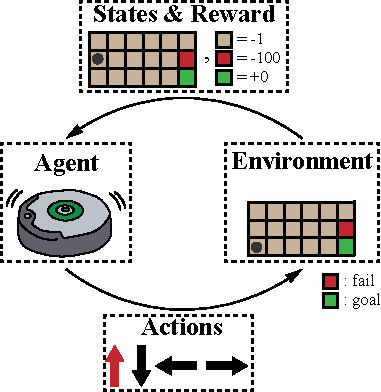
\includegraphics{reinforcement_learning_diagram.pdf}
	\caption{Reinforced learning framework for the application that a mobile robot must reach the desired position. In this example, the agent's actions are up, down, right and left; likewise, the agent's objective is reach the green cell and the agent fails when reach the red cell.}
	\label{fig:RL_framework}
\end{figure}

The framework of reinforcement learning is formed by four elements: (i) agent, (ii) actions, (iii) environment, and (iv) states and rewards \cite{sutton2018reinforcement}. Figure \ref{fig:RL_framework} describes the reinforcement learning framework for the application that a mobile robot must reach the desired position. First, an agent is the entity who takes decisions based on the reward and punishment that he will receive. Second, action space are all the available actions that the agent could use to interact with the environment. Third, the environment is the space where the agent lives and interact. Fourth,  the new agent's state after applying an action in the environment and the reward associated with that specific action. This process will be repeated several times until the agent learns a successful strategy to interact with the environment and maximize the reward.

In reinforcement learning, the agent's strategy is called policy ($\pi(s|a)$) and indicates which actions the agent should chooses in each state \cite{sutton2018reinforcement}. Policies are usually stochastic to consider the uncertainties and probabilities of real world \cite{tedrake2004stochastic}.  In this way, policies assign a probability of success to each action, and the agent chooses the action with the highest probability. Hence, the objective of reinforcement learning algorithms is to find the optimal policy that maximizes the amount of reward. 

The sum of the accumulated rewards from an initial state $s_t$ is the standard way of quantifying how good or bad the policy is \cite{sutton2018reinforcement}. This quality parameter is called value function ($V^{\pi}(s_t)$) and indicates the discounted sum of rewards that an agent will obtain starting in state $s_t$ and following the policy $\pi$ \cite{sutton2018reinforcement}. The value function can be computed as
\begin{equation*}
	V^{\pi}(s_t= s) = E_{\pi}  \left[r_t + \gamma r_{t+1} + \gamma^{2} r_{t+2}+ . . . | s_t = s \right],
\end{equation*}
\noindent where $r_t$ is the reward at time $t$, $\gamma$ is a discounted term and $s_t$ is the initial agent's state. However, calculating the value function requires the agent to start in all available states of the environment and in complex activities this can require a large amount of storage and computational cost. For this reason, more recent work uses deep neural networks to estimate the value function and optimal policy \cite{henderson2018deep}.

\begin{figure*}[t]
	\centering
	\subfloat[]{\includegraphics{policy_cnn.pdf}}
	\hfill
	\subfloat[]{\includegraphics{value_function_cnn.pdf}}
	\caption{Deep neural networks scheme: (a) predict optimal action and (b) estimate value function.}
	\label{fig:rl_cnn}
\end{figure*}

\section{Deep reinforcement learning}
Deep reinforcement learning (DRL) represent the combination of deep neural networks with reinforcement learning framework \cite{li2017deep}. Deep neural networks estimate the value function and predict the policy actions considering the agent's state as input. Figure \ref{fig:rl_cnn} describes the policy and value function parameterized with a neural network. Therefore, the goal of DRL is to find the neural network parameters that describe the optimal policy that generates the highest reward.

The policy gradient method optimizes the parameters of a neural network that define the behavior of the policy, and in this way, maximize the accumulated reward \cite{sutton2018reinforcement}. The policy gradient algorithms formulate an objective function related to the accumulated reward and then use the gradient ascent method to modify the parameters of the neural network~\cite{thomas2017policy}. The general form of the objective functions of the policy gradient algorithms is given by
\begin{equation*}
	L(\theta) = \expectation \left[ \mathrm{log} \pi_\theta (a|s) \advantage  \right],			
\end{equation*}
with,
\begin{equation*}
	\advantage = V^{\pi_{\theta}}_{t}  - \hat{V}_{t}, 
\end{equation*}
\noindent where $L(\theta)$ is the objective function, $\pi_\theta (a|s)$ is policy parameterized with neural network parameters ($\theta$), $\advantage$ is advantage function, $V^{\pi_{\theta}}_{t}$ is accumulated reward following policy $(\pi_\theta)$ and $\hat{V}_{t}$ is expected accumulated reward by the neural network.


\section{Proximal policy optimization}
PPO is a recent policy gradient method that strikes a good balance between rapid implementation and efficiency \cite{schulman2017proximal}. The PPO algorithm seeks to maximize accumulated reward, minimize estimation error of value function and explore different sequence of actions. Likewise, the PPO algorithm adds upper and lower limits to avoid large modifications of the neural network parameters \cite{schulman2017proximal}. In this way, PPO increases stability and reduces oscillations during neural network training.

The main objective function of PPO algorithm is given by
\begin{equation*}
	L^{\mathrm{CLIP}}(\theta) = \expectation \left[ \mathrm{min} \left(  r_{t}(\theta)  \advantage,  \mathrm{clip} (r_{t}(\theta) , 1-\epsilon, 1+\epsilon) \advantage  \right)  \right],	
\end{equation*}
with,
\begin{equation*}
	r_{t}(\theta) =\ratio,			
\end{equation*}
\noindent where $r_{t}(\theta)$ is the probability ratio between new and old policies, $\mathrm{clip}(\cdot)$ is the clip function to limit upper and lower increments, and $\epsilon$ is an hyperparameter that usually is  $0.2$ \cite{schulman2017proximal}.


The complete objective function of PPO algorithm can be computed as
\begin{equation*}
	L^{\mathrm{PPO}}(\theta) = \expectation \left[  L^{\mathrm{CLIP}}(\theta) - c_1 L^{\mathrm{VF}}(\theta)  + c_2 S[\pi_\theta](s_t)  \right],			
\end{equation*}	
with,
\begin{equation*}
	L^{\mathrm{VF}}(\theta) = \left( V_\theta (s_t) - V^{\mathrm{target}}_{t}  \right)^{2},	
\end{equation*}			
\noindent where $L^{\mathrm{CLIP}}(\theta)$ is the main objective function, $c_{1,2}$ are hyperparameters, $L^{\mathrm{VF}}(\theta)$ is square-error loss and $S$ is an entropy term to increase exploration \cite{schulman2017proximal}.

\section{Experimental setup}

\subsection{Bipedal robot simulation}
The legged robot has two legs (right and left). Likewise, each leg has three joints (ankle, knee, hip) and one joint for trunk orientation. Therefore, the robot has $14$ states considering position and velocity. Finally, the dynamic behavior of the bipedal robot is computed with the Multi-Joint dynamics with Contact (MuJoCo) physics simulator \cite{todorov2012mujoco}. Figure \ref{fig:bipedal_robot} describe the bipedal robot in a simulation environment of MuJoCo simulator.

\begin{figure}
	\centering
	\includegraphics{bipedal_robot.pdf}
	\caption{Bipedal robot in MuJoCo simulator. In this simulation environment, the robot has a trunk, left and right legs. Likewise, three joints in each leg (ankle, knee and hip).}
	\label{fig:bipedal_robot}
\end{figure}	

\subsection{Reinforcement learning: reward configuration}
The algorithm must learn to balance the robot as it moves forward. In this sense, the algorithm must receive positive reward based on the time that it maintains the balance when walking. Hence a simple way to set up the reward system is to give positive reward until the robot loses its balance. On the one hand, we establish that the robot loses its balance when the trunk's angular position is greater than $50^{\circ}$. On the other hand, the robot receives a positive reward of +1 for each iteration that maintains balance and a reward equal to the magnitude of the linear speed of the whole body to encourage forward movement.
